\chapter{Исследовательская часть}

\section{Технические характеристики}

Характеристики используемого оборудования:
\begin{itemize}
    \item Микроконтроллер STM32F303 с ОЗУ 48Кб, процессор  до 72 Мгц \cite{bib1}
\end{itemize}

\section{Время выполнения алгоритмов}

В таблице \ref{tbl:time_measurements} приведено время выполнения алгоритмов для разных
квадратных матриц. На рисунке \ref{fig:images-Figure_1} показаны графики
выполнения алгоритмов умножения матриц в тиках процессора.

\begin{table}[h]
	\begin{center}
		\begin{threeparttable}
		\captionsetup{justification=raggedright,singlelinecheck=off}
		\caption{Время работы алгоритмов (в тиках процессора)}
		\label{tbl:time_measurements}
		\begin{tabular}{|c|r|r|r|r|}
			\hline
			Размер матриц &  Классический & Виноград & Виноград оптимизированный \\
			\hline
                        2 & 0.98 & 0.75 & 0.73 \\ \hline 
                        3 & 0.83 & 0.79 & 0.74 \\ \hline 
                        4 & 1.01 & 0.90 & 0.90 \\ \hline 
                        5 & 1.18 & 1.15 & 1.23 \\ \hline 
                        6 & 1.68 & 1.56 & 1.50 \\ \hline 
                        7 & 2.10 & 2.00 & 2.05 \\ \hline 
                        8 & 2.80 & 2.46 & 2.49 \\ \hline 
                        9 & 3.72 & 3.21 & 3.36 \\ \hline 
                        10 & 5.60 & 4.18 & 5.36 \\ \hline 
                        10 & 5.04 & 4.50 & 4.50 \\ \hline 
                        21 & 41.45 & 30.15 & 31.04 \\ \hline 
                        32 & 143.91 & 91.93 & 90.18 \\ \hline 
                        43 & 316.11 & 213.24 & 218.61 \\ \hline 
                        54 & 592.50 & 367.35 & 403.39 \\ \hline 
                        65 & 937.01 & 608.54 & 620.80 \\ \hline 
                        76 & 1531.09 & 960.95 & 967.34 \\ \hline 
                        87 & 2216.74 & 1423.29 & 1448.46 \\ \hline 
                        98 & 3178.86 & 2044.33 & 2059.81 \\ \hline 
                        109 & 4462.48 & 2832.23 & 2927.09 \\ \hline 
		\end{tabular}
		\end{threeparttable}
    \end{center}
\end{table}


\clearpage

\begin{figure}[h]
    \centering
    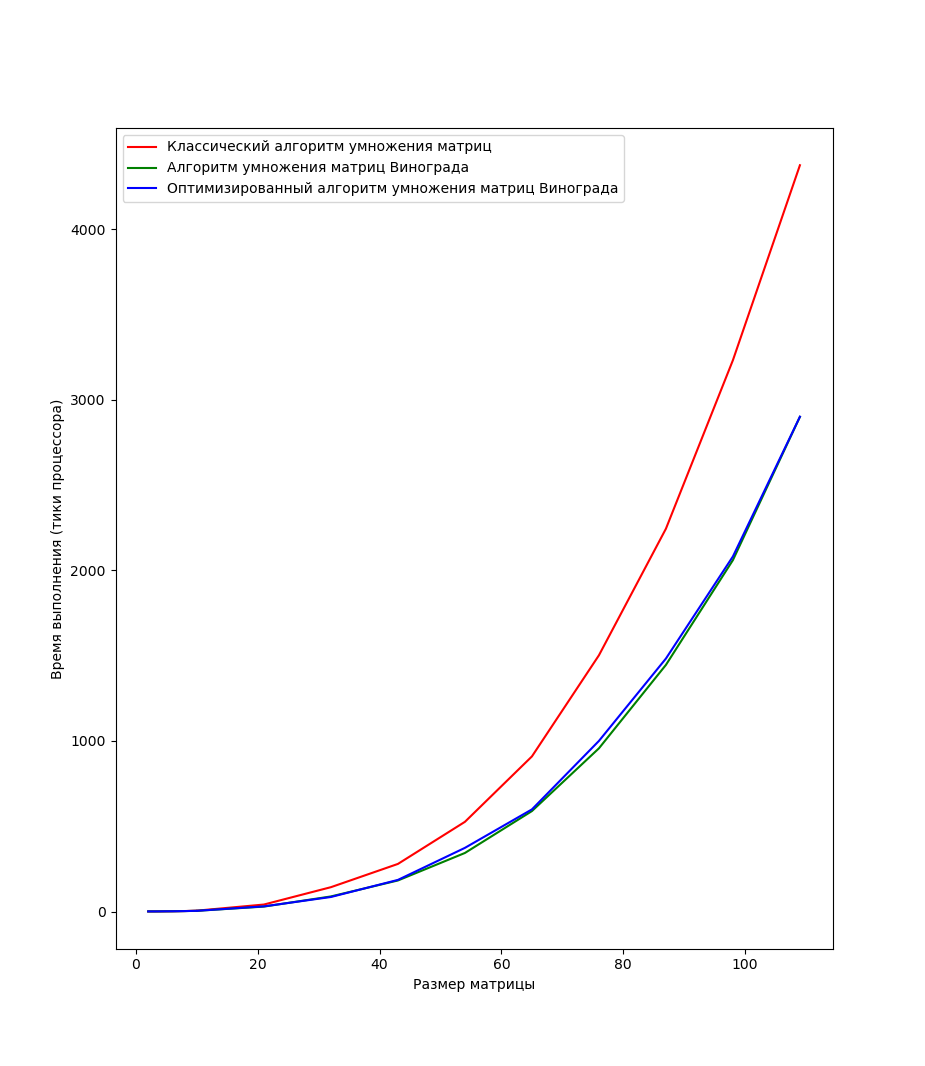
\includegraphics[width=0.8\textwidth]{images/Figure_1}
    \caption{Графики в тиках процессора}
    \label{fig:images-Figure_1}
\end{figure}

\section{Вывод}

Сравнения проводились на квадратных матрицах четного и нечетного размеров. Во всех случаях
классический алгоритм проигрывает алгоритму Винограда по количеству необходимых тиков
процессора на выполнения задачи. Оптимизированная и обычная версии алгоритма Винограда
используют довольно одинаковое количество тиков процессора, отчего можно сказать,
что их производительность примерно одинаковая. Возможно, это произошло по причие оптимизаций
компилятора.

